\documentclass{article}

\usepackage{tikz} 

\usepackage{amsmath} % advanced math

% margins of 1 inch:
\setlength{\topmargin}{-.5in}
\setlength{\textheight}{9.5in}
\setlength{\oddsidemargin}{0in}
\setlength{\textwidth}{6.5in}

\usepackage{hyperref}
\hypersetup{
    colorlinks=true,
    linkcolor=blue,
    filecolor=magenta,      
    urlcolor=cyan,
    pdftitle={Overleaf Example},
    pdfpagemode=FullScreen,
    }

\usepackage{graphicx}
\graphicspath{ {./images/} }
\usepackage{float}
\usepackage[demo]{graphicx}

\begin{document}

    % https://stackoverflow.com/a/3408428/1164295
        \title{2022 Future Computing Summer Internship Project:\\(Creating examples of Thundering Herd for the Structural Simulation Toolkit Discrete Event Simulator)}
        \author{Melissa Jost\thanks{melisssakjost@gmail.com}\ }
        \date{\today}
            \maketitle
        \begin{abstract}
            The focus of this project is to remedy the lack of examples of various distributed system
            design problems, and our ability to detect these issues.  Our goal within this repository was to use a simulation of \href{https://en.wikipedia.org/wiki/Thundering_herd_problem}{thundering herd} to come up with a set of metrics applicable to analyzing other systems.  More specifically, we simulated a scenario with users trying to access a website with a cache and a server within the \href{http://sst-simulator.org/}{Structural Simulation Toolkit (SST)}, and used different parameters of this problem to analyze if thundering herd had occurred.  The work within this repository is currently a work in progress.  While the bare bone work has been laid out for the simulation within SST, more can be done to refine this simulation to more closely mirror the interactions users have with websites within the real world, such as how long it would take for a cache to respond to one's request.  In addition, more research still has to be done in terms of defining a set of metrics to detect this problem, though some suggestions have been detailed in the paper.
        \end{abstract}

\ \\
% see https://en.wikipedia.org/wiki/George_H._Heilmeier#Heilmeier's_Catechism

%\maketitle

\section{Project Description} % what problem is being addressed? 

The challenge that is being addressed by this work is that while we have countless examples of what issues exist within distributed systems, as well as various ways to avoid them, there is still a lack of work that exists with regards to quantifying metrics to detect these issues.  
By creating these simulations, we provide concrete implementations of thundering herd, which can be helpful to both those working to better understand these issues, as well as those trying to understand how to use SST as a whole. 

\section{Motivation} % Why does this work matter? Who cares? If you're successful, what difference does it make?

The users of this work include two main groups of people: those developing distributed systems, and those interested in learning how to use SST.  This work benefits people developing distributed systems by specifying a useful set of metrics for detecting these various design problems, even if in simple simulations, it could potentially save a lot of time in finding them in real systems in the future.  For those learning SST, these simulations help give more, simple examples of how to use the toolkit.

\section{Prior work} % what does this build on?

Most of the prior work that we used so far focused on defining the problem at hand, and referencing real world instances of the thundering herd problem occurring so we knew how to define our simulation with SST.  First off, one important distinction that we needed to make was that between \href{https://en.wikipedia.org/wiki/Cache_stampede}{cache stampede} and thundering herd.  As discussed by a blog post by TechExpertise, cache stampede is a variant of the thundering herd problem. \cite{techexpertise}  Thundering herd occurs when a set of threads all want to request the same set of locked data, but their calls to wake up all become synchronized, meaning no one can get through.  When each thread all competes for this single resource at the same time, it could freeze up the system, causing issues.  In a cache stampede, this resource is usually an item in a cache.  All the threads request a value that isn't present, and when they receive a miss they all go to memory at the same time, once again causing the system to freeze up.  This summer, we decided focusing on this relationship between users and a cache would be most beneficial, so we chose to simulate a cache stampede.  

After we settled on a definition for thundering herd that we wanted to stick to, we had to find an example worth simulating in order for us to conduct our analysis of the problem.  An article by Sunny Beatteay detailing a real-world instance of the thundering herd problem helped point us in the right direction.\cite{beatteay}  This detailed the cause of a huge Facebook outage that occurred in 2010, where an invalid value within the site's database led to every user trying to fix the issue, overwhelming it with requests.  Beatteay explains that while it was a notable scenario for Facebook at the time, whose millions of users were unable to access the site for hours, it can occur at any level.  The problem scales with the amount of memory you have, so can occur for companies with smaller databases as well.  Based on this, we decided the best way to model this problem was to also simulate the interactions between clients and a website.

\section{How to do the thing}

% The software developed to respond to this challenge was run on (one laptop/a cluster of 100 nodes).

For the simulation, we are able to run it with one laptop, and it currently connects 5 users to a cache, and this cache to a server.  While this is how most of the current work was analyzed, this simulation could benefit from having a wider number of users connected to the cache in order to simulate the true "herd" of requests. By altering the number of users, in addition to the frequency in website requests or length of time to handle these requests, we could observe different scenarios.  \newline

The software is available \href{https://github.com/lpsmodsim/2022HPCSummer-ThunderingHerd}{here.}  To run the code, you need to run the Makefile.  An example of the output is shown below.
 \begin{verbatim}
make
mkdir -p .build
singularity exec /usr/local/bin/additions.sif g++ -std=c++1y -D__STDC_FORMAT_MACROS -fPIC 
-DHAVE_CONFIG_H -I/opt/SST/11.1.0/include -MMD -c diningPhilosopher.cc 
-o .build/diningPhilosopher.o
mkdir -p .build
singularity exec /usr/local/bin/additions.sif g++ -std=c++1y -D__STDC_FORMAT_MACROS -fPIC 
-DHAVE_CONFIG_H -I/opt/SST/11.1.0/include -MMD -c diningTable.cc -o .build/diningTable.o
singularity exec /usr/local/bin/additions.sif g++ -std=c++1y -D__STDC_FORMAT_MACROS -fPIC 
-DHAVE_CONFIG_H -I/opt/SST/11.1.0/include -shared -fno-common -Wl,-undefined 
-Wl,dynamic_lookup -o liblivelock2.so .build/diningPhilosopher.o .build/diningTable.o
singularity exec /usr/local/bin/additions.sif sst-register livelock2 
livelock2_LIBDIR=/home/mkjost/projects/livelock/2022HPCSummer-Livelock/diningTableExample
singularity exec /usr/local/bin/additions.sif sst tests/diningPhilosopher.py 
...
Text output in output.txt
Simulation statistics in CSV files
Simulation is complete, simulated time: 150 Ks
 \end{verbatim}

\section{Model} % how are we modeling this within SST?

Our simulation has 3 main components: websiteUsers, a websiteCache, and a websiteServer.  Each of the users have a port to the cache, and the cache connects to the server.  Currently, we manually define each of these users within the Python file, but in the future we'd like to make it easier to scale the amount of users within the simulation.  Below, we have a visualization of what the simulation looks like when 5 users are present. \newline

\begin{figure}[H]
    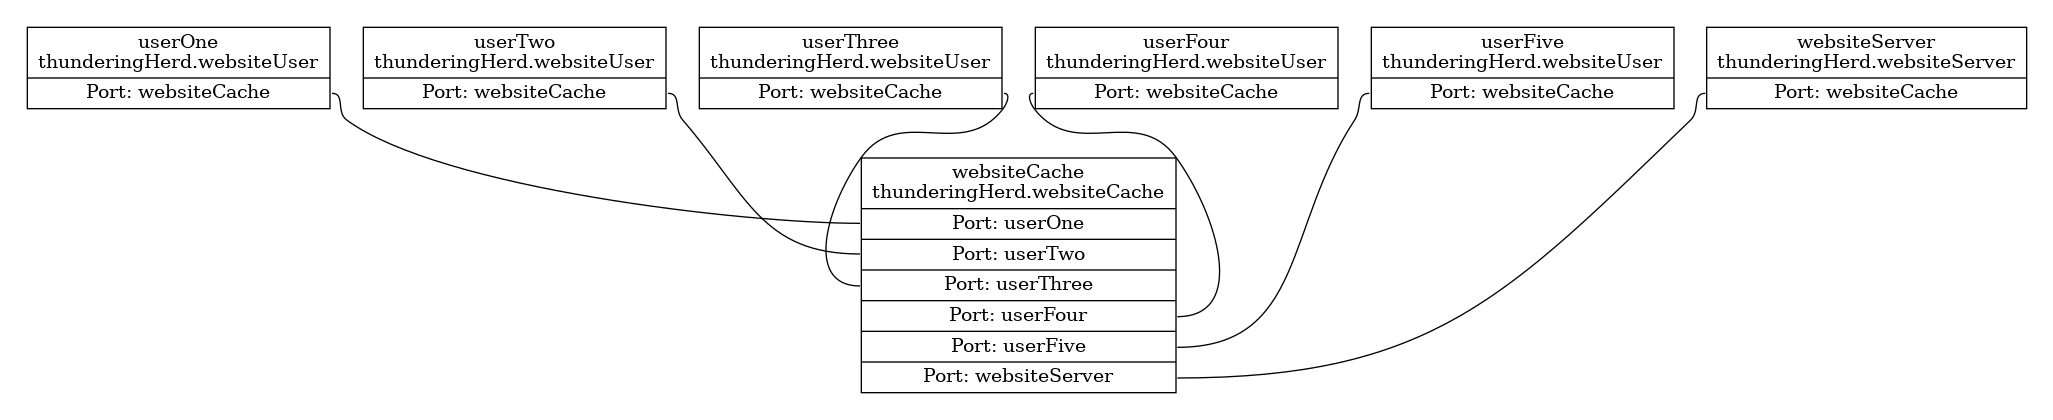
\includegraphics[scale=0.22]{images/thunderingHerd.png}
    \caption{Visualization of Component Connections within Thundering Herd Simulation}
\end{figure}

The general timeline of events that the simulation follows starts out with the user requesting to visit a certain website.  The user has a knowledge of the names of pages it can access, but not the physical page that the server holds.  We randomize a request to the cache for one of these pages, and once the cache receives it, it adds the request to a queue that gets handled every cycle.  \newline

Once the cache is ready to handle this event, it checks its own internal map to see if it has a copy of the requested page already saved.  If it does, it sends it back to the user, who switches to a browsing state in which they stay occupied on the same page for a certain amount of cycles.  However, if the page isn't within the cache, the cache will have to send a request to the server for the page, and update the user that the page isn't stored within it yet.  \newline

The servers only functionality is to receive requests from the cache, push them onto its own queue, and process them every cycle.  The difference between the cache and the server is that the server takes longer to process requests.  In addition, the server holds access to all the physical pages, and these pages are defined at the beginning of the simulation. \newline

Once the cache hears back from the server, it has to update its internal state with a cache replacement policy.  Within this simulation, we chose to implement the Least Recently Used (\href{https://en.wikipedia.org/wiki/Cache_replacement_policies#Least_recently_used_(LRU)}{LRU}) policy.  If the cache is full, we'll loop through all the values within the cache, locating the element that was accessed the longest time ago.  From here, we'll delete that element, then add in the page that was requested.  In addition, once we update the cache, we can also send a message back to the user that the page they were requesting was ready. \newline

However, if there's a delay in sending this message back to the user and its request times out, the user will enter a waiting state, in which they become impatient in their wait for the requested page.  At this point, they'll begin to send more frequent requests to the cache, mirroring users constantly refreshing pages when they fail to load.  The idea behind this behavior is that if all users request the same page that isn't within the cache at the same time, their waiting states will also trigger at the same point, sending synchronized waves of requests to slow down the server \newline

Within this simulation, the main things one can configure using parameters is the amount of time each of these message requests take.  You can define how long it will take for the cache to process each request on its queue, as well as the length of time for the server to process requests.  We can also define how long it will take a user's request to timeout, leading to them entering their waiting state.  In the future, we hope to parameterize the amount of users within the simulation as well. \newline

\section{Result} % conclusion/summary

The results of our simulation at this point is that we have some ideas of how to formulate metrics for this problem that still need to be looked into more.  For example, when running simulations, we noticed once we added a queue to both our server and cache, it was easier to see the increase in requests added to the queue as more users started sending multiple requests for the same website.  In addition, similar to other distributed system problems we've looked at this summer, we could potentially compare the amount of request timeouts, or the amount of time the waitingTick function in the user is actively used in order to detect thundering herd issue.  However, one thing we have to note is that for the thundering herd issue to occur, all users would have to simultaneously request the same site, so we'd need a way to differentiate this specific behavior from a general problem where the server was overloaded with random requests.

\section{Future Work} % what needs to be done now?

Since the simulation of this problem is still a work in progress, there is a lot of work that can be done with it in the future.  One step that can be taken is to tweak the current model so that it more closely models the interactions one would normally observe between a user and a website.  For example, we'd want to make sure the amount of time spent handling a cache request or a server request was realistic.  In addition, we'd want to make sure that the size of the cache is proportionate to the amount of data within the server, and that all of these values properly scale with an increase in users. \newline

On that note, we would also want to rework this simulation so that scaling the amount of users is a parameter that can easily be increased.  At the moment, each user is individually defined, along with its specific port to the cache.  Our simulation only has 5 users, so modelling a realistic example of thundering herd can't be done just yet. Ideally, we'd want hundreds of users all requesting the same value from the cache at the same time, so increasing the users would be helpful for future analysis. \newline

Once the simulation has been tweaked accordingly, we could analyze the results of various simulations in order to come up with a set of metrics to detect the thundering herd problem.  At the moment, the main statistics we've been observing during the creation of this simulation was the queue size of both the cache and server, as well as the frequency with which each user sends re-requests.  However, as stated above, we need to make sure we differentiate between issues occurring to a high number of differing requests to the server, and issues occurring because all users are requesting the same exact value from the server. \newline

Lastly, this analysis could also benefit from more research in terms of defining the problem, as cache stamepede and thundering herd have been used interchangeably in the sources we referred to this summer.  Looking for more research into this problem could give more insight as to how to alter our simulations, in addition to giving us more information as to what data would be best analyzed to create our metrics. 

\begin{thebibliography}{9}
\bibitem{texbook}
Donald E. Knuth (1986) \emph{The \TeX{} Book}, Addison-Wesley Professional.

\bibitem{lamport94}
Leslie Lamport (1994) \emph{\LaTeX: a document preparation system}, Addison
Wesley, Massachusetts, 2nd ed.

\bibitem{beatteay}
Sunny Beatteay (2021) \emph{\href{https://betterprogramming.pub/how-a-cache-stampede-caused-one-of-facebooks-biggest-outages-dbb964ffc8ed}{How a Cache Stampede Caused One of Facebook’s Biggest Outages}}, Medium. 

\bibitem{techexpertise}
TechExpertise (2021) \emph{\href{https://serantechexplore.wixsite.com/website/post/multithreading-thundering-herd-cache-stampede-and-lock-convoy-problems}{Multithreading: Thundering herd, Cache stampede and Lock convoy problems}}
\end{thebibliography}

\end{document}